\begin{frame}[hoved]
	\frametitle{Evaluation}
	\begin{minipage}[t]{0.45\textwidth}
		{\large Debugging}
		\begin{itemize}
			\item Debugging using the riscv32-unknown-elf-gdb debugger.
			\item Able to see the different cores active as "Threads".
			\item Connects to the QEMU virtual machine remotely.
		\end{itemize}
	\end{minipage}
	\hfill
	\begin{minipage}[t]{0.45\textwidth}
		\begin{figure}
			\begin{center}
				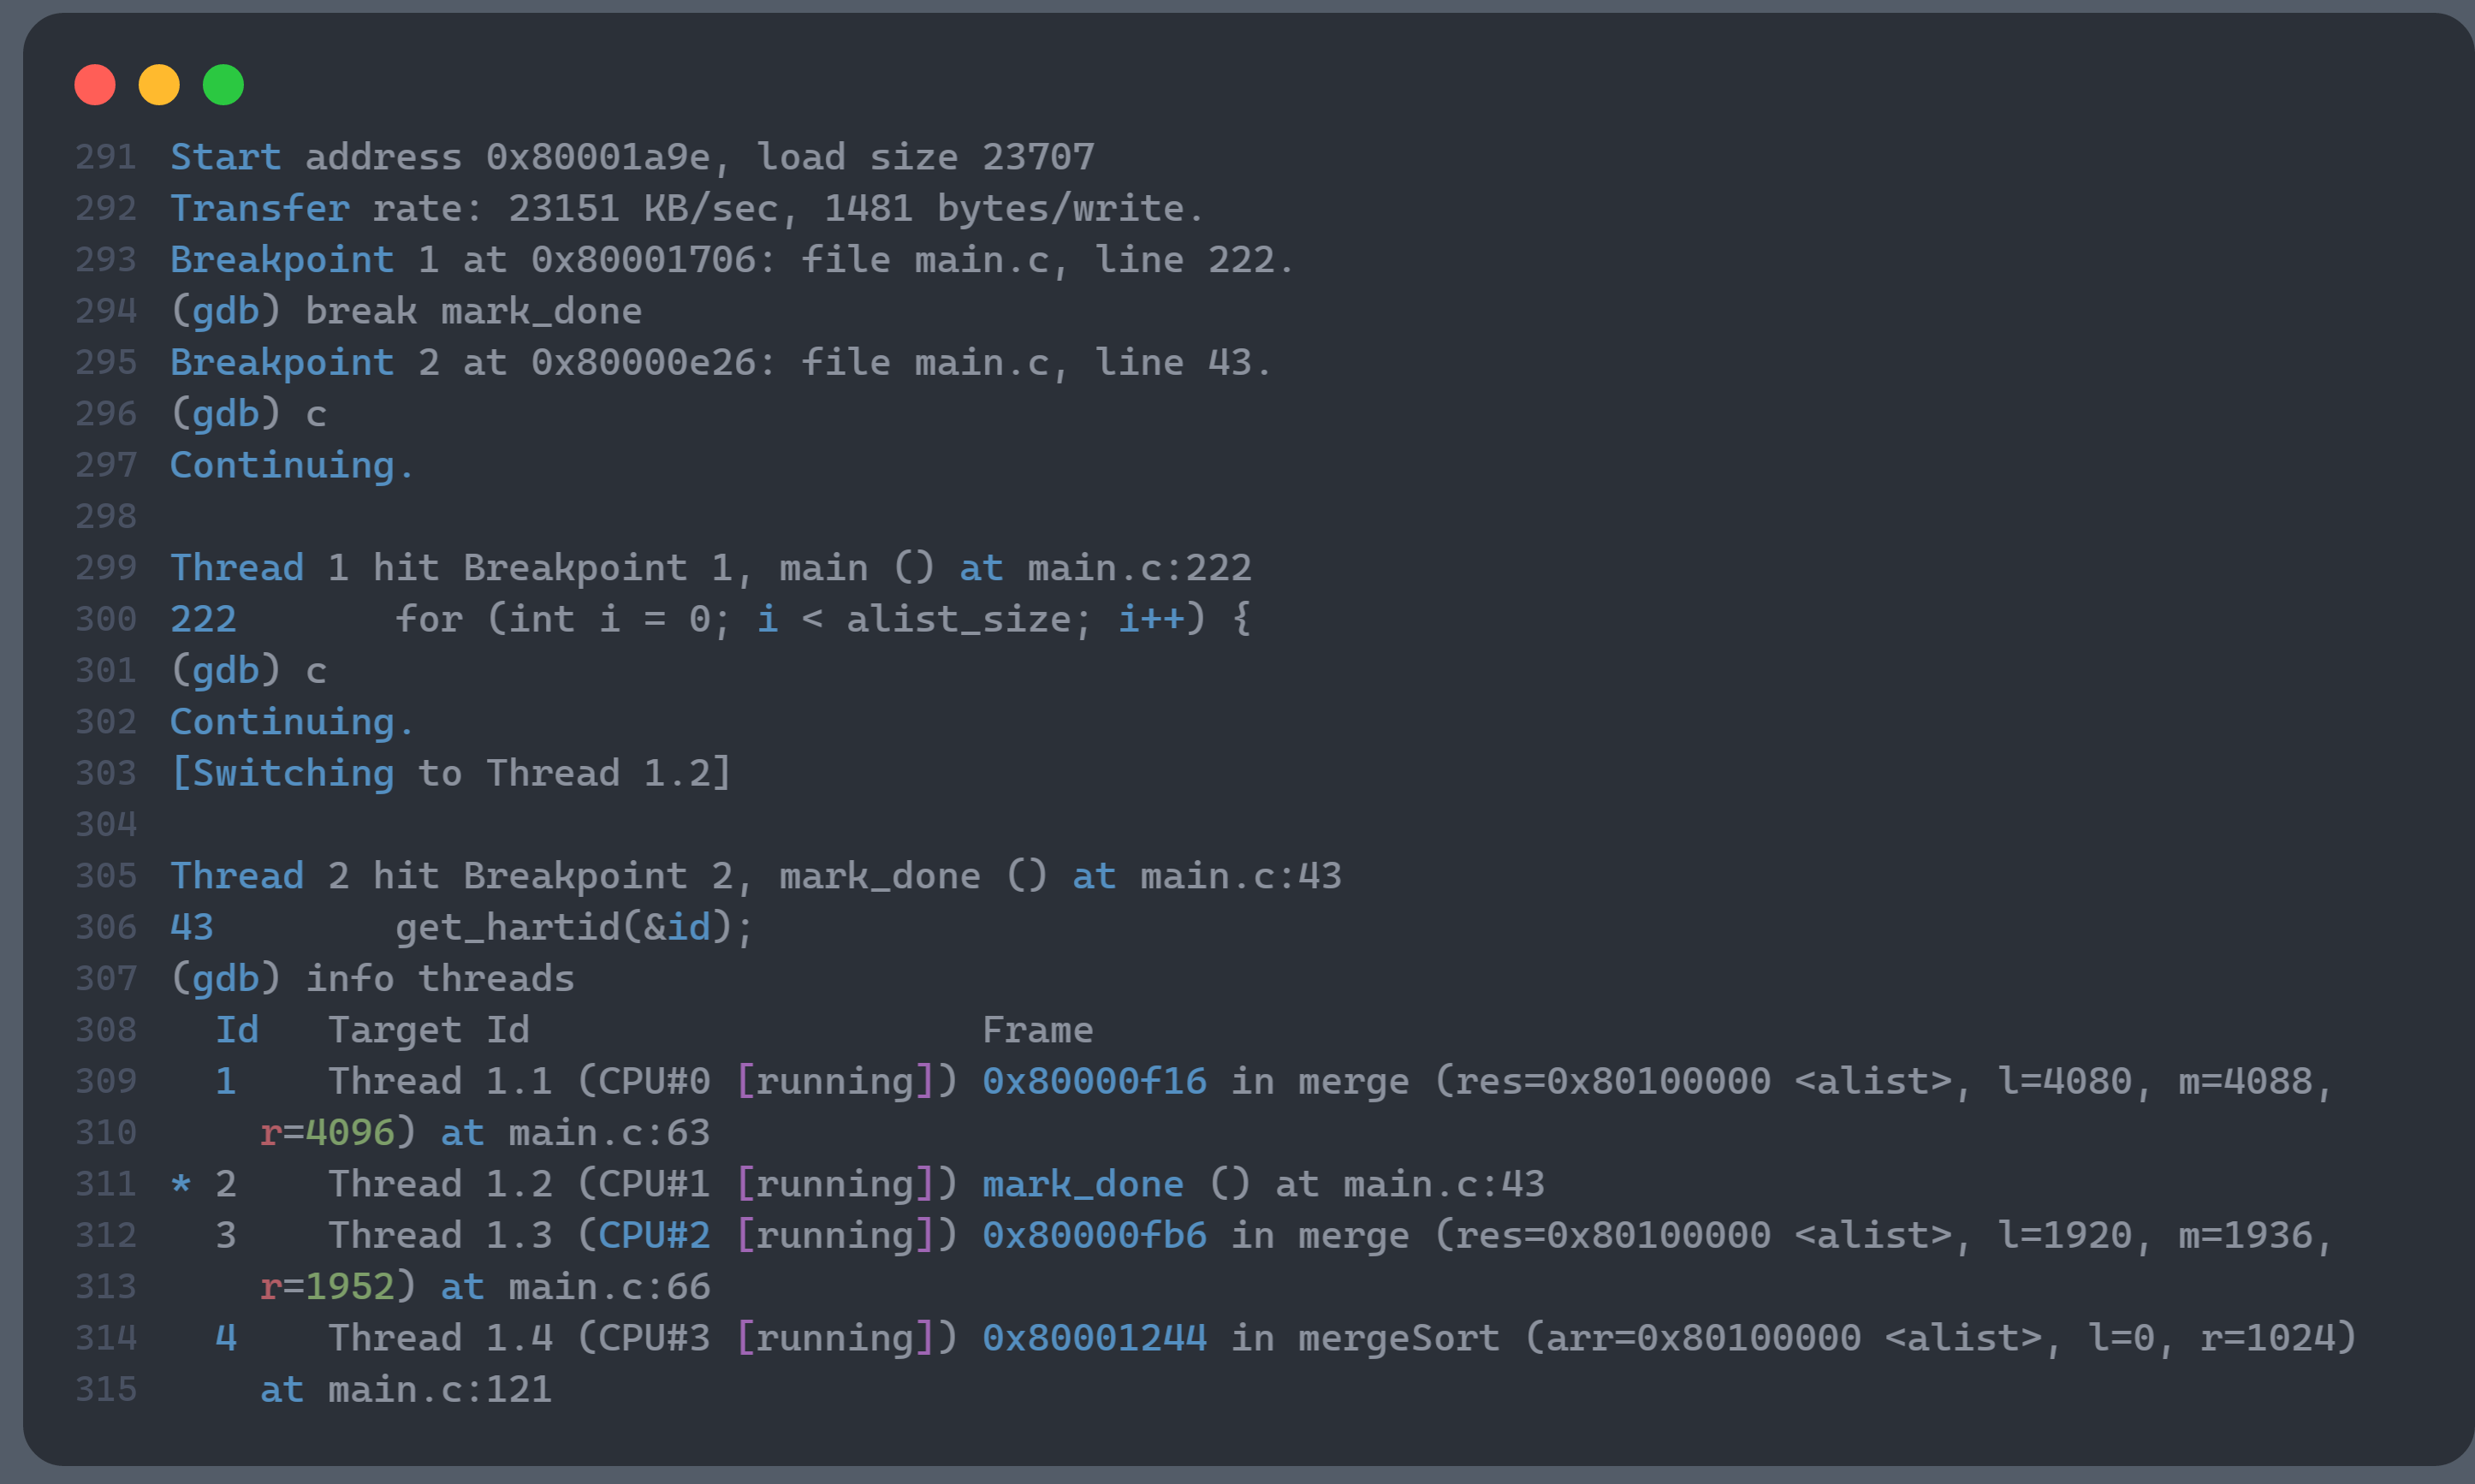
\includegraphics[width=0.95\textwidth]{figures/debugging.png}
			\end{center}
			\caption{Debugging}\label{fig:debugging}
		\end{figure}
	\end{minipage}
\end{frame}

\begin{frame}[hoved]
	\frametitle{Evaluation}
	\begin{minipage}[t]{0.45\textwidth}
		{\large Validation}
		\begin{itemize}
			\item Tested using varying sizes.
			\item Redirects QEMU stdout to file and compares with python sort.
			\item Found that number of cores has to be less than list size.
			\item Number of cores has to be a power of 2. Due to the partitioning.
		\end{itemize}
		{\large Future work}
		\begin{itemize}
			\item Variable thread stack size.
			\item Performance testing. QEMU emulates number of cores.
		\end{itemize}
	\end{minipage}
	\hfill
	\begin{minipage}[t]{0.45\textwidth}
		\begin{figure}
			\begin{center}
				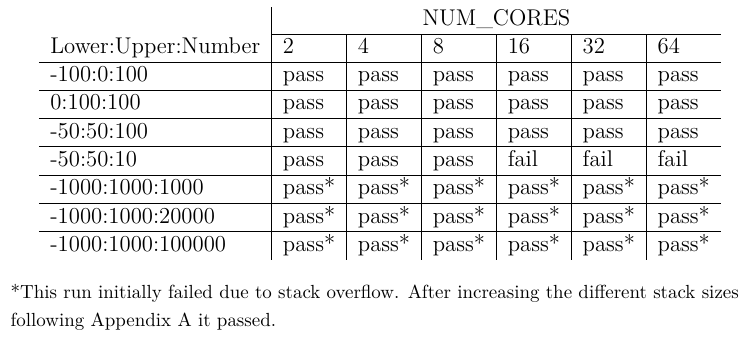
\includegraphics[width=0.95\textwidth]{figures/validate.png}
			\end{center}
			\caption{Lists of varying sizes tested}\label{fig:validate}
		\end{figure}
	\end{minipage}
\end{frame}
